%%%%%%%%%%%%%%%%%%%%%%%%%%%%%%%%%%%%%%%%%
% Lachaise Assignment
% LaTeX Template
% Version 1.0 (26/6/2018)
%
% This template originates from:
% http://www.LaTeXTemplates.com
%
% Authors:
% Marion Lachaise & François Févotte
% Vel (vel@LaTeXTemplates.com)
%
% License:
% CC BY-NC-SA 3.0 (http://creativecommons.org/licenses/by-nc-sa/3.0/)
% 
%%%%%%%%%%%%%%%%%%%%%%%%%%%%%%%%%%%%%%%%%

%----------------------------------------------------------------------------------------
%	PACKAGES AND OTHER DOCUMENT CONFIGURATIONS
%----------------------------------------------------------------------------------------

\documentclass{article}

%%%%%%%%%%%%%%%%%%%%%%%%%%%%%%%%%%%%%%%%%
% Lachaise Assignment
% Structure Specification File
% Version 1.0 (26/6/2018)
%
% This template originates from:
% http://www.LaTeXTemplates.com
%
% Authors:
% Marion Lachaise & François Févotte
% Vel (vel@LaTeXTemplates.com)
%
% License:
% CC BY-NC-SA 3.0 (http://creativecommons.org/licenses/by-nc-sa/3.0/)
% 
%%%%%%%%%%%%%%%%%%%%%%%%%%%%%%%%%%%%%%%%%

%----------------------------------------------------------------------------------------
%	PACKAGES AND OTHER DOCUMENT CONFIGURATIONS
%----------------------------------------------------------------------------------------

\usepackage{amsmath,amsfonts,stmaryrd,amssymb} % Math packages

\usepackage{enumerate} % Custom item numbers for enumerations

\usepackage[ruled]{algorithm2e} % Algorithms

\usepackage[framemethod=tikz]{mdframed} % Allows defining custom boxed/framed environments

\usepackage{listings} % File listings, with syntax highlighting
\lstset{language=C,keywordstyle={\bfseries \color{blue}}}

%----------------------------------------------------------------------------------------
%	DOCUMENT MARGINS
%----------------------------------------------------------------------------------------

\usepackage{geometry} % Required for adjusting page dimensions and margins

\geometry{
	paper=a4paper, % Paper size, change to letterpaper for US letter size
	top=2.5cm, % Top margin
	bottom=3cm, % Bottom margin
	left=2.5cm, % Left margin
	right=2.5cm, % Right margin
	headheight=14pt, % Header height
	footskip=1.5cm, % Space from the bottom margin to the baseline of the footer
	headsep=1.2cm, % Space from the top margin to the baseline of the header
	%showframe, % Uncomment to show how the type block is set on the page
}

%----------------------------------------------------------------------------------------
%	FONTS
%----------------------------------------------------------------------------------------

\usepackage[utf8]{inputenc} % Required for inputting international characters
\usepackage[T1]{fontenc} % Output font encoding for international characters

\usepackage{XCharter} % Use the XCharter fonts

%----------------------------------------------------------------------------------------
%	COMMAND LINE ENVIRONMENT
%----------------------------------------------------------------------------------------

% Usage:
% \begin{commandline}
%	\begin{verbatim}
%		$ ls
%		
%		Applications	Desktop	...
%	\end{verbatim}
% \end{commandline}

\mdfdefinestyle{commandline}{
	leftmargin=10pt,
	rightmargin=10pt,
	innerleftmargin=15pt,
	middlelinecolor=black!50!white,
	middlelinewidth=2pt,
	frametitlerule=false,
	backgroundcolor=black!5!white,
	frametitle={Command Line},
	frametitlefont={\normalfont\sffamily\color{white}\hspace{-1em}},
	frametitlebackgroundcolor=black!50!white,
	nobreak,
}

% Define a custom environment for command-line snapshots
\newenvironment{commandline}{
	\medskip
	\begin{mdframed}[style=commandline]
}{
	\end{mdframed}
	\medskip
}

%----------------------------------------------------------------------------------------
%	FILE CONTENTS ENVIRONMENT
%----------------------------------------------------------------------------------------

% Usage:
% \begin{file}[optional filename, defaults to "File"]
%	File contents, for example, with a listings environment
% \end{file}

\mdfdefinestyle{file}{
	innertopmargin=1.6\baselineskip,
	innerbottommargin=0.8\baselineskip,
	topline=false, bottomline=false,
	leftline=false, rightline=false,
	leftmargin=2cm,
	rightmargin=2cm,
	singleextra={%
		\draw[fill=black!10!white](P)++(0,-1.2em)rectangle(P-|O);
		\node[anchor=north west]
		at(P-|O){\ttfamily\mdfilename};
		%
		\def\l{3em}
		\draw(O-|P)++(-\l,0)--++(\l,\l)--(P)--(P-|O)--(O)--cycle;
		\draw(O-|P)++(-\l,0)--++(0,\l)--++(\l,0);
	},
	nobreak,
}

% Define a custom environment for file contents
\newenvironment{file}[1][File]{ % Set the default filename to "File"
	\medskip
	\newcommand{\mdfilename}{#1}
	\begin{mdframed}[style=file]
}{
	\end{mdframed}
	\medskip
}

%----------------------------------------------------------------------------------------
%	NUMBERED QUESTIONS ENVIRONMENT
%----------------------------------------------------------------------------------------

% Usage:
% \begin{question}[optional title]
%	Question contents
% \end{question}

\mdfdefinestyle{question}{
	innertopmargin=1.2\baselineskip,
	innerbottommargin=0.8\baselineskip,
	roundcorner=5pt,
	nobreak,
	singleextra={%
		\draw(P-|O)node[xshift=1em,anchor=west,fill=white,draw,rounded corners=5pt]{%
		Question \theQuestion\questionTitle};
	},
}

\newcounter{Question} % Stores the current question number that gets iterated with each new question

% Define a custom environment for numbered questions
\newenvironment{question}[1][\unskip]{
	\bigskip
	\stepcounter{Question}
	\newcommand{\questionTitle}{~#1}
	\begin{mdframed}[style=question]
}{
	\end{mdframed}
	\medskip
}

%----------------------------------------------------------------------------------------
%	WARNING TEXT ENVIRONMENT
%----------------------------------------------------------------------------------------

% Usage:
% \begin{warn}[optional title, defaults to "Warning:"]
%	Contents
% \end{warn}

\mdfdefinestyle{warning}{
	topline=false, bottomline=false,
	leftline=false, rightline=false,
	nobreak,
	singleextra={%
		\draw(P-|O)++(-0.5em,0)node(tmp1){};
		\draw(P-|O)++(0.5em,0)node(tmp2){};
		\fill[black,rotate around={45:(P-|O)}](tmp1)rectangle(tmp2);
		\node at(P-|O){\color{white}\scriptsize\bf !};
		\draw[very thick](P-|O)++(0,-1em)--(O);%--(O-|P);
	}
}

% Define a custom environment for warning text
\newenvironment{warn}[1][Warning:]{ % Set the default warning to "Warning:"
	\medskip
	\begin{mdframed}[style=warning]
		\noindent{\textbf{#1}}
}{
	\end{mdframed}
}

%----------------------------------------------------------------------------------------
%	INFORMATION ENVIRONMENT
%----------------------------------------------------------------------------------------

% Usage:
% \begin{info}[optional title, defaults to "Info:"]
% 	contents
% 	\end{info}

\mdfdefinestyle{info}{%
	topline=false, bottomline=false,
	leftline=false, rightline=false,
	nobreak,
	singleextra={%
		\fill[black](P-|O)circle[radius=0.4em];
		\node at(P-|O){\color{white}\scriptsize\bf i};
		\draw[very thick](P-|O)++(0,-0.8em)--(O);%--(O-|P);
	}
}

% Define a custom environment for information
\newenvironment{info}[1][Info:]{ % Set the default title to "Info:"
	\medskip
	\begin{mdframed}[style=info]
		\noindent{\textbf{#1}}
}{
	\end{mdframed}
} % Include the file specifying the document structure and custom commands

%----------------------------------------------------------------------------------------
%	ASSIGNMENT INFORMATION
%----------------------------------------------------------------------------------------

\title{CS426: Project \#1 Report} % Title of the assignment

\author{Doruk Çakmakçı\\ \texttt{21502293}} % Author name and email address

\date{Bilkent University --- \today} % University, school and/or department name(s) and a date

%----------------------------------------------------------------------------------------

\begin{document}

\maketitle % Print the title

%----------------------------------------------------------------------------------------
%	INTRODUCTION
%----------------------------------------------------------------------------------------

\section{Implementation and Design Decisions} % Unnumbered section
\qquad In this project, serial and parallel programs that solve  matrix multiplication and compute sum were implemented. As the first step, the serial programs that solve the mentioned problems were implemented. Then, these programs are converted to parallel programs without discarding the main algorithmic approaches to the problem. MPI(Message Passing Interface) is used for applying parallel programming principles to the problems. Matrix multiplication problem is solved with a single parallel program that uses Send & Receive functions of MPI. On the other hand, compute sum problem is solved using two different parallel approaches: One-to-One communication(Send and Receive operations) and Collective Communication(Broadcast, Reduce and Barrier operations). In the following sections, the implementation and the design decisions important for the implementation are explained in detail.

\subsection{Compute Sum}

\subsubsection{Serial Program for Compute Sum}
\qquad This program consists of two straightforward steps: Reading the input file using file operations of C and computing the sum of the numbers read from file. The input file is read using \lstinline{fgets}function of C. While reading the file, each number is summed to an accumulator variable. Since there is a chance of overflow while summing numbers, the accumulator is declared as long long type instead of int type.

\subsubsection{Parallel Program for Compute Sum using One-to-One Communication Between Nodes}
\qquad This program is a parallel version of the serial implementation of the compute sum program described above. In this program, master processor reads the file, distributes numbers to the available processors according to the ratio of the number of processors and the length of numbers to sum. Then, the workers compute the local sum of their portions and send the results to the master. The master computes the sum of the received data and prints result to the console. For this implementation, master reads the input file two times, for finding the count of numbers to sum and distributing the numbers to the available processors. Instead of reading the file twice, the numbers to sum could be stored for distribution to workers but since the count of numbers is not known beforehand, we needed a dynamic sized data storage instead of a static sized one. Since reading the file twice is a more straightforward approach, it is followed. If the input file is too large, the currently used approach may introduce a more significant overhead compared to the dynamic re-sizing of the data structure to be used. The One-to-One communication scheme used is as follows: First, master sends the size of the portion assigned to workers(can be different for each processor). The worker receives the size of the portion and allocates corresponding space to store the numbers. Then master sends the corresponding portion to each worker. The workers receive their portion and sums the numbers. The workers send the results to the master processor. Note that master processor also does computation. Finally, master sums the received data and prints the result to the console. Even though the timing of the sends and receives can differ, there can not be race conditions between the operations mentioned since MPI\_Receive is a blocking receive operation(at least for a time interval). However, this program can be made more efficient by sending portion sizes using collective communication(Broadcast) and by reducing the local sums to the master processor using Reduce operation. But this part is defined only to use One-to-One communication between processors so these improvements can not be done. Also note that master processor also does computation.

\subsubsection{Parallel Program for Compute Sum using Collective Communication Between Nodes}
\qquad This program is a different parallel version of the serial compute sum program. Collective communication operations of MPI is used instead of one-to-one communication. All processors execute the same code snippet except the file operations are only done by the master processor. The implementation pipeline is as follows: First, master processor reads the file line by line twice. At the first read, the line count is stored. At the second read, the numbers themselves are stored to an array. After the numbers are stored in the memory, master processor broadcasts the line count to worker processors. Then, worker processors allocate space to store the numbers. After receiving the line count, master sends all of the array to the worker processors for further computation. An MPI\_Barrier is used to guarantee that all processors finish the operations until now. Then, all processors compute the quotient and the remainder of division between number count and the number of processors. The quotient and remainder is used to compute the location and size of the portion of the array to sum. All processors sum their portion. At the end, MPI\_Allreduce is used to reduce the local sums computed to all processors whilst summing them to generate the global sum. Now, all processors have the global sum in their storage. This program can be made more efficient by not only using collective communication but also using one-to-one communication. Instead of passing all of the array elements to every processor, the corresponding array chunks could be passed to each processor separately. This solution decreases both the space allocated per processor and communication overhead(sending a very large data vs small sized data). 

\subsection{Matrix Multiplication}

\subsubsection{Serial Program for Matrix Multiplication}
\qquad This program consists of reading 2 matrices from different files to the memory, multiplying the matrices and writing the result to a separate file. All steps were straightforward. The standard matrix multiplication algorithm is used for matrix multiplication. The running time of this program could be improved by using divide and conquer solution for matrix multiplication or Strassen's algorithm. The standard algorithm is used because it is easier to create a parallel implementation using this algorithm.

\subsubsection{Parallel Program for Matrix Multiplication}
\qquad The parallel version of the serial program mentioned above uses only one-to-one communication between processors. The implementation pipeline is as follows: First of all master reads matrices from file to two dimensional arrays. The first matrix is read normally but, the second matrix is read from the file in a transposed manner( so that rows of the matrix become the columns  of the matrix). This decision makes separating the matrix to blocks of rows and columns much easier since after transpose operation. Also the 1-D block distribution becomes much more easier to implement. Then, master processor computes the computation to be made per processor and sends block sizes to worker processors. Now for the computation part, master computes it's portion first then the turn for computation passes to other processors. Each processor computes it's portion  one at a time. Workers send results to master and master writes results to file. The detailed explanation of the pipeline is written as comments to the program. This program could also use collective communication for some operations(passing the computation per node and block size from master to worker processors). However, this change does not induce a great speedup. 

\section{Implementation Testing and Results}

\subsection{Graphs}
\qquad The matrix multiplication programs are run with the inputs sent with the email. The compute sum programs are run with a file that contains numbers from 1 to 50(inclusive). For the serial programs, the interval for timing measurements are between the start of the main and end of the main. For the parallel programs the interval for timing measurements are between MPI\_Init() and MPI\_Finalize(). The matrix multiplication programs are run with  1,4,9,25,36 and 100 processing nodes for testing. The compute sum programs are run with 1, 2, 3, 5, 10, 20, 30, 50, 75 and 100 processing nodes for testing purposes. The runtime of the program versus the number of thread graphs are provided as Figure 1. \\

\begin{figure}
\centering
\begin{minipage}{.5\textwidth}
  \centering
  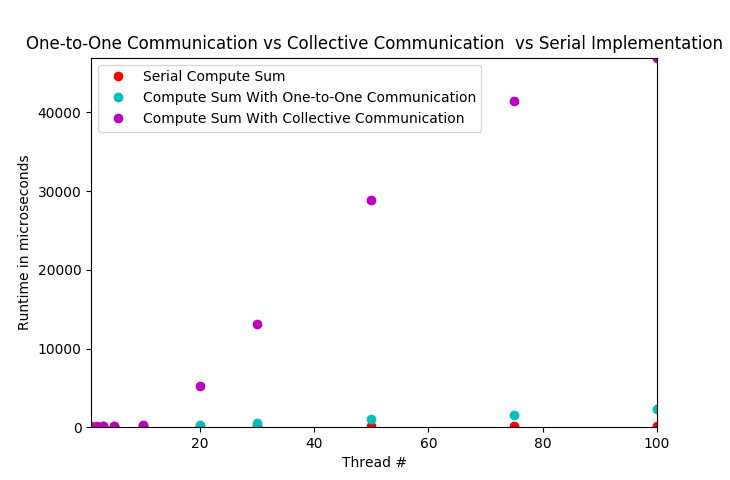
\includegraphics[width=\linewidth]{assets/compute_sum.png}
  \label{fig:test1}
\end{minipage}%
\begin{minipage}{.5\textwidth}
  \centering
  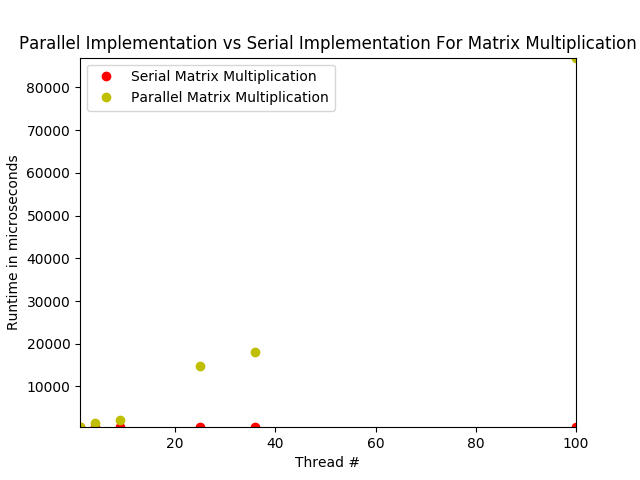
\includegraphics[width=\linewidth]{assets/mm.png}
  \label{fig:test2}
\end{minipage}
\vspace{-2}
\caption{Comparison of Implementations}
\end{figure}

\quad The runtimes(in micro seconds) used for creating the plot is below:
\begin{itemize}
    \item {Serial Compute Sum: 204}
    \item {Parallel Compute Sum Version 1: 79, 75, 134, 101, 227, 367, 574, 1045, 1615, 2284}
    \item {Parallel Compute Sum Version 2: 28, 68, 128, 196, 288, 5249, 13188, 28850, 41399, 46966}
    \item {Serial Matrix Multiplication: 532}
    \item {Parallel Matrix Multiplication: 468, 1374, 2053, 14864, 18055, 86970}
\end{itemize}
\qquad In the graphs we see the runtimes of different implementations of both problems compared to the number of threads used. In both cases, the runtime of the serial implementation does not depend on the number of threads. Also, from the graphs we see that the runtime of the algorithms does not always improve with increasing number of threads. At some point(depending on the input size), increasing the number of threads do not provide enough speed-up compared to the burden of communication between processors. Also, the runtime is highly dependent to the current situation of the process nodes used. As expected, the runtimes of the programs were fluctuating with respect to the run. Also, another point to note, when the parallel implementations of either problems are run with 1 nodes, the results seem to be better than the serial implementation. This may be due to the difference in the checkpoints used for measuring time for different implementations. Regarding the both schemes, the tests are done with not-so-large inputs. The results can highly differ with respect to the input size. \\
\null\qquad According to the timing measurements, the parallel implementations of compute sum are faster than the serial implementation of compute sum when the number of threads are less then 5. Also the runtime of the parallel versions up to 5 processing nodes are not stable and the average of the results of all implementations seem to be similar. On the other hand, when the thread number is large, there is a significant performance difference between all compute sum implementations. The implementation that uses collective communication has a significantly worse performance compared to the One-to-One communication implementation. This result is expected because while the collective communication scheme passes the array as whole to worker processes, One-to-One scheme passes the array by dividing it to the chunks that only contain the data to be used by the worker processor. Therefore, the redundant communication overhead of sending the redundant array elements is avoided in one-to-one communication scheme. \\
\null\qquad According to the timing measurements, the parallel implementation of matrix multiplication is faster than serial implementation up to 2 threads. If the thread numbers increase further, the overhead of creating and connecting processor nodes and communication between processors slows the program down significantly. For this implementation, even when 2 threads are used, the communication overhead significantly slows down the program. \\


\end{document}
